\section{Aturan Dasar Penulisan Kode PHP}
Seperti bahasa pemograman yang lain, PHP juga memiliki aturan penulisan seperti case sensitifity (perbedaan antara huruf besar dan kecil), cara mengakhiri sebuah baris perintah, dan pengaruh penggunakan spasi dalam membuat kode program PHP. Berikut adalah aturan dasar penulisan kode PHP:
\subsection{Case Sensitivity (perbedaan huruf besar dan kecil) dalam PHP}
PHP tidak membedakan huruf besar dan kecil (case insensitive) untuk penamaan fungsi (function), nama class, maupun keyword bawaan PHP seperti echo, while, dan class. Ketiga baris berikut akan dianggap sama dalam PHP:
\begin{lstlisting}
<?php
Echo “Hello World”;
ECHO “Hello World”;
EchO “Hello World”;
?>
\end{lstlisting}
Akan tetapi, PHP membedakan huruf besar dan huruf kecil (case sensitive) untuk penamaan variabel, sehingga akan dianggap sebagai variabel yang berbeda. Sering kali error terjadi dikarenakan salah menuliskan nama variabel, yang seharusnya menggunakan huruf kecil, ditulis dengan huruf besar.
\begin{lstlisting}
<?php
$luqman="Luqman";
echo $Luqman; // Notice: Undefined variable: Luqman
?>
\end{lstlisting}
Untuk mengatasi perbedaan ini, disarankan menggunakan huruf kecil untuk seluruh kode PHP, termasuk variabel, fungsi maupun class. Jika membutuhkan nama variabel yang terdiri dari 2 kata, karakter spasi bisa digantikan dengan underscore.
\subsection{Karakter Spasi dan Tab dalam PHP}
Dalam PHP, karakter seperti spasi dan tab diabaikan di dalam eksekusi program PHP. Anda boleh mencoba sebuah statement menjadi beberapa baris, atau menyatukan beberapa statement dalam sebuah baris yang lumayan panjang. Seperti contoh berikut:
\begin{lstlisting}
<?php
echo "Saya belajar"; echo "Saya mengerti"; $nama="Men";
?>
\end{lstlisting}
Baris statement itu sama dengan
 \begin{lstlisting}
<?php
     echo "Saya belajar";
     echo "Saya mengerti";
     $nama = "Men";
?>
\end{lstlisting}
Walaupun contoh yang pertama lebih menghemat baris, namun lebih disarankan untuk contoh kedua, karena kita mengusahakan agar setiap statement berada dalam satu baris saja, dan menambahkan beberapa spasi di awal untuk memudahkan membaca kode program.
\par
Keuntungan penghematan baris dan beberapa byte dari sebuah file PHP tidak akan sebanding dengan mencoba memahami kode program yang dibuat dalam beberapa hari kedepan. Menambahkan sebagian komentar pada bagian kode yang lebih rumit sebagai penjelasan juga sangat disarankan.
\section{Embedded Script dan Non Embedded}
\subsection{Embedded Script}
  \item Berikut merupakan contoh dokumen HTML yang akan dihasilkan dengan menggunakan program/script PHP dalam embedded script
    Ditampilkan dibawah ini  :
    \lstinputlisting[firstline=1, lastline=12]{src/embedded_script.php}
Script diatas menunjukkan contoh script PHP sederhana yang disebut dengan script embedded yang di sisipkan diantara tag-tag HTML. Script tersebut digunakan apabila isi dari suatu dokumen HTML diinginkan dari hasil eksekusi suatu script PHP. jika dilihat dari source-nya dengan menggunakan view source pada web browser maka tampilannya akan berupa seperti berikut
    \lstinputlisting[firstline=14, lastline=22]{src/embedded_script.php}
Source dokumen HTML yang tampil berupa dokumen HTML yang tidak lagi dari script PHP yang berisi script PHP karena semua menjadi tag HTML, karena pada saat dieksekusi maka bukan scriptnya yang dikirim tetapi eksekusi dari script tersebut yang dikirim 
\subsection{Non Embedded}
   \item Script PHP dibawah ini merupakan script murni dari pembuatan program dengan menggunakan PHP, tag dokumen HTML yang dihasilkan untuk membuat dokumen merupakan bagian dari script PHP. di tampilkan dibawah ini:
  \lstinputlisting[firstline=24, lastline=35]{src/embedded_script.php}
dan dibawah ini merupakan source dokumen HTML dari tampilan kode diatas  
  \lstinputlisting[firstline=38, lastline=40]{src/embedded_script.php}
Jika diperhatikan dokumen HTML tersebut tidak beraturan ditampilkan. Hal tersebut tidak menjadi masalah, yang penting adalah browser web dapat menampilkannya, karena dokumen tag HTML ini murni dihasilkan dari script PHP. 

\section{Variabel dan Tipe Data}
\subsection{Variabel}
Variabel adalah tempat penympanan data, variabel memiliki nama. dalam pemograman variabel merupakan tempat penyimpanan data didalam memori komputer. Didalam PHP nama variabel diawali dengan karakter dollar diikuti dengan huruf sebagai karakter pertama setelah dollar. kemudian kombinasi karakter dan angka. Tidak boleh ada spasi dan tanda baca dalam penamaannya. kecuali karakter (garis bawah, under score).berikut merupakan penulisan variabel yang benar:
\lstinputlisting[firstline=31, lastline=34]{src/tag_awal_akhir.php}
\begin{lstlisting}
<?php
$npm="1154054";
$nama=' Luqman Nurfajri';
echo"npm : ".npm ."<br>;
echo"nama: &nama";
?>
\end{lstlisting}

\subsection{Tipe Data}
Data yang diolah oleh suatu program memiliki berbagai jenis ada data yang menunjukkan jumlah dan menunjukkan nilai benar dan salah, atau tulisan. Jenis tipe data dalam PHP secara mendasar dibedakan menjadi 3 macam yang disebut sebagai tipe data primitif. Tipe data primitif yang diolah oleh PHP:
\begin{enumerate}
\item Numerik
\item String
\item Boolean
\end{enumerate}
Tipe data numerik dibedakan menjadi tipe data integer dan flooting point. Selain itu tipe data yang lain adalah tipe data compound, terdiri atas:
\begin{enumerate}
\item Tipe Data Array
\item Tipe Data Objek 
\end{enumerate}

\subsection{Tipe Data Integer}
Tipe data integer adalah tipe data yang terdiri dari angka bulat (tidak mengandung nilai pecahan atau nilai desimal). Nilai ini bisa berbentuk angka positif maupun negatif, contohnya 1, 2, 6, -44, 20000, atau 128730123. Tipe data integer dapat dituliskan dengan notasi sebagai berikut
\begin{enumerate}
\item Notasi Desimal adalah susunan bilangan yang mempunyai basis sepuluh. 
Koefisien bilangan desimal terdiri dari 0,1,2,3,4,5,6,7,8,9.
Notasi bilangan desimal dituliskan: (n)10
\item Notasi Oktal adalah susunan bilangan yang mempunyai basis delapan. 
Koefisien bilangan oktal terdiri dari 0,1,2,3,4,5,6,7.
Notasi bilangan oktal dituliskan : (n)8
\item Biner adalah susunan bilangan yang mempunyai basis dua. 
Basis dua di sini adalah nilai koefisien yaitu 0 dan 1.
Notasi bilangan biner dituliskan : (n)2
\item Notasi Heksadesimal adalah susunan bilangan yang mempunyai basis enam belas. 
Koefisien bilangan heksadesimal terdiri dari 0,1,2,3,4,5,6,7,8,9,A,B,C,D,F.

Catatan: A bernilai 10, B bernilai 11, ... , F bernilai 15.
Notasi bilangan hekasdesimal dituliskan : (n)16

\begin{figure}[!htbp]
 \centering
 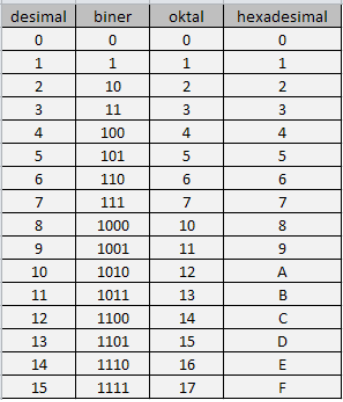
\includegraphics[width=.50\textwidth]{figures/sistem_bilangan.png}
 \caption{Sistem Bilangan}\label{fig:inputchapter}
\end{figure}
\end{enumerate}

\subsection{Tipe Data Floting Point}
Tipe data float (disebut juga tipe data floating point, atau real number) adalah tipe data angka yang memiliki bagian desimal di akhir angka, atau memiliki floating point (floating point adalah istilah dalam bahasa inggris untuk menyebut tanda “titik” yang menandakan bilangan desimal). Contoh angka float adalah seperti: 0,9 atau 3,14. Tipe data float cocok digunakan untuk variabel yang akan berisi angka pecahan, seperti nilai IPK, hasil pembagian, atau hasil komputasi numerik yang angkanya tidak bisa ditampung oleh data integer.
\subsection{Tipe Data String}
Tipe data String adalah tipe data untuk teks yang merupakan gabungan huruf, angka, whitespace (spasi), dan berbagai karakter. Fungsi ini digunakan untuk membuat identifier String/teks. Data string ditulis dengan mengapit data string tersebut dengan tanda petik tunggal atau tanda petik ganda. Tanda petik tunggal umumnya digunakan sebagai konstanta string.
\subsection{Tipe Data Boolean}
Tipe data boolean sebenarnya sangat sederhana. Tipe data ini hanya bisa diisi dengan salah satu dari 2 nilai: TRUE atau FALSE. Tipe data boolean banyak dipakai dalam percabangan kode program, atau untuk memutuskan apa yang harus dijalankan pada sebuah kondisi if else.
\subsection{Tipe Data Objek}
Tipe data dari objek merupakan tipe data baru, merupakan pengembangan PHP untuk mendukung program berorientasi objek. Tipe data objek adalah tipe data yang didalamnya mempunyai data dan method. data yang dipunyai oleh suatu objek populer dengan nama atribut dan method suatu objek umumnya berupa suatu fungsi. 

Data objek didefinisikan dengan membuat definisi kelas terlebih dahulu. Suatu variabel yang bertipe objek diinisialisasi (dideklarasi) dengan menggunakan perintah new kemudian nama objek (berupa nama kelas objek) berikut contohnya:
\lstinputlisting[firstline=1, lastline=17]{src/tipeDataObjek.php}


\section{Operator PHP}
Pada PHP, terdapat banyak operator  beberapa yang sering digunakan.
\subsection{Operator Perbandigan}
Seperti namanya, operator perbandingan digunakan untuk membandingkan beberapa buah nilai pada PHP dan hasilnya berupa booelan true yang berarti benar atau false yang berarti salah.
Contoh:
\begin{lstlisting}
<?php
if ($_POST['password'] == 'admin')
{
	echo 'Login sukses';
}
\end{lstlisting}

\subsection{Operator PHP Increment dan Decrement}
Operator ini digunakan untuk menambahkan atau mengurangi nilai sebanyak 1 pada suatu variabel. 
\subsection{Perbedaan Pre Increment dan Post Increment}
Pada pre increment, nilai variabel akan ditambahkan 1 baru kemudian siap digunakan, sebaliknya, untuk  post increment, gunakan dulu nilai variabel kemudian baru ditambahkan dengan 1.
Contoh 1:
\begin{lstlisting}
<?php
$nomor = 1;
while($nomor <= 5) {
	echo $nomor++;
}
\end{lstlisting}
Contoh diatas akan menghasilkan angka 12345.

Contoh 2:
\begin{lstlisting}
<?php
$nomor = 1;
while($nomor <= 5) {
	echo ++$nomor;
}
\end{lstlisting}
Contoh diatas akan menghasilkan 23456.
Lihat, perbedaanya terdapat pada ++ sebelum dan sesudah $nomor. 

\subsection{Operator Assignment PHP}
Sesuai namanya operator assignment ini digunakan untuk memberikan nilai pada suatu variabel. Operator dasarnya adalah tanda sama dengan ( = ). Dalam praktiknya, operator ini sering digunakan ketika menjumlahkan nilai pada suatu perulangan, seperti ketika menjumlahkan data hasil query database.
Contoh:
\begin{lstlisting}
<?php
$sql 	= 'SELECT * FROM sales';
$query 	= mysqli_query($sql);
$total	= 0;
while($row = mysqli_fetch_array($query))
{
	$total += $row['jml_bayar'];
}
?>
\end{lstlisting}


\section{Lingkup Variabel}
Variabel Scope (atau ruang lingkup variabel) adalah jangkauan kode program dimana perintah program masih bisa mengakses sebuah variabel. Variabel menunjukkan keberlakuan dan dikenalinya suatu variabel didalam script. Suatu variabel yang didefinisikan didalam sebuah fungsi maka variabel tersebut hanya akan dikenali dan digunakan hanya dalam fungsi tersebut variabel ini dikenal sebagai variabel lokal. karena hanya dikenal pada fungsi tempat variabel tersebut dinyatakan dan digunakan.

Jika kita mendefenisikan sebuah variabel pada satu file PHP, maka variabel tersebut dapat diakses oleh seluruh kode program pada halaman yang sama. Namun jika variabel tersebut di defenisikan di dalam sebuah fungsi, variabel itu belum tentu bisa diakses dari luar fungsi tersebut. Hal inilah yang dimaksud dengan Variabel Scope. Variabel akan disebut global apabila variabel tersebut dapat dikenali dan digunakan oleh seluruh bagian script tersebut

Variabel yang didefenisikan di dalam sebuah fungsi, secara default tidak dapat diakses oleh kode program di luar fungsi tersebut. Dan begitu juga sebaliknya, variabel yang didefenisikan di luar fungsi, tidak bisa diakses dari dalam fungsi. Berikut jenis variabel berdasarkan lingkupnya:

\subsection{Variabel Global}
Variabel dan nilainya dikenali dan dapat digunakan oleh semua bagian script yang membutuhkannya. Semua variabel yang dibuat pada bagian utama script bukan pada bagian suatu fungsi, variabel variabel ini akan bersifat global. Pengertian global disini diartikan sebagai variabel dan data yang ada didalamnya hanya dikenali oleh seluruh bagian script, jika script dieksekusi oleh PHP.

Fungsi-fungsi yang ingin menggunakan variabel dan data yang ada pada variabel global, maka dalam fungsi harus dideklarasikan global untuk nama variabel tersebut

contohnya:
\lstinputlisting[firstline=1, lastline=14]{src/lingkupVariabel.php}

Variabel array global merupakan variabel asosiatif internal PHP yang mencatat semua variabel global yang dimiliki oleh suatu script. Proses penggunaan suatu variabel global dalam suatu fungsi dapat memanfaatkan array  berikut contohnya:
\lstinputlisting[firstline=16, lastline=26]{src/lingkupVariabel.php}
agar variabel dan data didalamnya dapat dipakai oleh script-script yang saling berhubungan dan membutuhkan maka variabel harus dinyatakan dengan cookie, method GET, ataupun method POST.

\subsection{Variabel Lokal}
Variabel lokal adalah variabel dan data yang dimilikinya hanya dapat digunakan oleh fungsi tempat variabel digunakan dideklarasikan.
Nama variabel bisa memiliki nama yang sama dengan nama variabel global yang ada pada script, tetapi tetap yang diacuh oleh fungsi adalah variabel lokal.
Variable jenis ini di tulis di dalam function, dan hanya dapat di akses dari dalam function juga, dengan kata lain tidak bisa di akses di luar function, berikut contoh syntax nya :
\lstinputlisting[firstline=31, lastline=44]{src/lingkupVariabel.php}
Syntax diatas dapat terlihat jelas, jika Variable Local di akses di dalam function maka nilainya keluar yakni ‘5’, sedang jika di akses diluar function maka nilai itu tidak ada.

\subsection{Variabel Statik}
Variabel statik dalam fungsi yang memungkinkan nilai yang terahir yang ada didalamnya dapat dipertahankan, karena secara biasa sertiap fungsi selesai dieksekusi, pada saat dipanggil kembali nilai yang ada pada variabel dalam fungsi tersebut akan diinisialisasi lagi. Pernyataan static memungkinkan nilai yang terahir dipertahankan, sehingga pada saat dipanggil kembali fungsi tersebut masih memiliki nilai yang terahir. Biasanya ketika sebuah function selesai di jalankan dalam sebuah syntax PHP, semua variable di dalamnya akan di hapus, namun terkadang kita ingin agar variable tersebut tidak di hapus, akan tetapi akan kita gunakan secara lanjut, untuk itu kita harus menggunakan variable statis dalam case ini, berikut syntax nya :
\lstinputlisting[firstline=48, lastline=63]{src/lingkupVariabel.php}
Perbedaan dengan jenis variable lain ialah terletak, jika setiap function dipanggil, nilai yang ada di dalam variable adalah nilai terakhir, bukan nilai yang di deskripsikan seperti syntax diatas yakni ‘8’.


\section{Struktur Kontrol}
PHP melakukan eksekusi dengan perintah mulai dari baris pertama kemudian ke baris berikutnya, sampai baris yang terakhir. Struktur kontrol digunakan dalam mengatur alur logika program agar sesuiai dengan kenyataan. Struktur kontrol akan melibatkan variabel, tipe data, dan operator. 
\subsection{If Statement}
If Statement  adalah pernyataan yang hanya akan dijalankan jika suatu kondisi bernilai benar, berfungsi untuk melakukan filter/penyaringan hasil berdasarkan kondisi tertentu. Contoh:
Kondisi IF adalah kondisi dimana sebuah data yang apabila kondisinya jika dan hanya nilai kebenaran dari hasil yang dibuat adalah benar, tetapi jika kondisi yah diuji salah maka sistem / program akan tidak menanggapi. Contoh:
\begin{lstlisting}
 if (bebas) {
                pernyataan benar
}
\end{lstlisting}
Dari skrip diatas parameter IF ini dapat kita gunakan dalam PHP, buatlah file dengan nama \textbf{bebas.php}.
\begin{lstlisting}
<html>
<head>
<title> Test Kondisi IF </title>
   <body>
    <?php
         $bebas ="aih";

         if ($bebas == "aih") {
                echo "Buku ini semoga bermanfaat";
          }
         ?>
    </body>
</html>
\end{lstlisting}

\subsection{Perulangan}
\subsubsection{Struktur Kondisi IF ELSE}
Kondisi IF ELSE  digunakan untuk jika kondisi kita memiliki dua pilihan dari hasil yang berbeda, contohnya hasil yang keluar bernilai benar (\textit{true}) dan bernilai salah (\textit{false}). Secara standar sintaks seperti ini:
\begin{lstlisting}
if (bebas) {
    statement benar
} else {
     statement salah
}
\end{lstlisting}
Dari sintaks diatas kita dapat menyimpulkan bahwa, apabila \textbf{bebas} mendapatkan nilai yang sesuai maka \textit{statement} akan benar maka program yang akan dieksekusi benar dan jika \textbf{bebas} mendapatkan nilai salah maka yang dieksekusi adalah \textit{statement} salah. Berikut contoh penggunaan kondisi IF dan ELSE. Buatlah file dengan nama\textbf{ ifelse.php}:
\begin{lstlisting}
<html>
<head>
<title>Test Kondisi IF dan ELSE </title>
</head>
    <body>
        <?php
            $makan = "eat";
                 if ($makan=="eat")
                      echo "Makan adalah bahasa indonesia dari eat";
                 else {
                      echo "Makan bukan bahasa indonesia dari EAt";
                  }
          ?>
    </body>
</html>
\end{lstlisting}

\subsubsection{Struktur Kondisi Switch Dan Case}
Struktur kondisi SWITCH DAN CASE digunakan saat penyelesaian dari persoalan dengan jumlah kondisi yang banyak. Struktur ini dapat memeriksa nilai suatu variabel dengan SWITCH dan memeriksa kondisi dengan CASE. Contoh:
\begin{lstlisting}
switch ($var) {
case '1' : statement-1; break;
case '2' : statement-2; break;
....
}
\end{lstlisting}
Berikut contoh penggunaan kondisi SWITCH dan CASE. Buatlah file dengan nama\textbf{ swicase.php}:
\begin{lstlisting}
<?php
$day =date ("D");
switch ($day) {
    case 'Sun' : $hari= "Minggu" ; break;
    case 'Mon' : $hari= "Senin" ; break;
    case 'Tue' : $hari= "Selasa" ; break;
    case 'Wed' : $hari= "Rabu" ; break;
    case 'Thu' : $hari= "Kamis" ; break;
    case 'Fri' : $hari= "Jum'at" ; break;
    case 'Sat' : $hari= "Sabtu" ; break;
    default: $hari = "Kiamat" ;
}
echo "Hari ini hari <b>$hari</b>";
?>
\end{lstlisting}

\subsubsection{Struktur Perulangan For}
Struktur perulangan digunakan dalam kondisi membatasi perulangan. sebagai contoh disini kita mengulang kalimat "Semoga buku ini bermanfaat" sebanyak 50 kali. Buatlah file dengan nama \textbf{for.php}
\begin{lstlisting}
<?php
for ($i= 1; $i <= 50; $i++)
{
   echo "Semoga buku ini bermanfaat";
   echo "<br />";
}
?>
\end{lstlisting}

\subsubsection{Struktur Perulangan While}
Struktur perulangan while digunakan pada saat banyaknya perulangan tidak dapat kita pastikan.
Disini kita mengulang angka  1 sampai 14 sebagai contoh:  Buatlah file dengan nama \textbf{while.php}
\begin{lstlisting}
<?php
$i=1;
while ($i <= 14)
{
  echo "$i";
  echo "<br />";
  $i=$i+1;
}
?>
\end{lstlisting}

\subsubsection{Struktur Perulangan Do While}
Struktur Do While sebenernya lanjutan dari perulangan While, perbedaan keduanya dilihat dari posisi pengecakan kondisi. Apabila perulangan While kondisi yang dicek di awal maka perulangan Do While di akhir perulangan. Disini kita mengulang angka  1 sampai 14 sebagai contoh:  Buatlah file dengan nama \textbf{dowhile.php}
\begin{lstlisting}
<?php
$i=1;
do
{
  echo "$i";
  echo "<br />";
  $i=$i+1;
} while ($i <= 10);
?>
\end{lstlisting}

\subsubsection{Struktur Perulangan Foreach}
Array adalah sebuah tipe data yang sering digunakan dalam membuat program menggunakan PHP. Kemampuan array dalam menyimpan banyak data dalam satu variabel akan sangat berguna untuk menyederhanakan dan menghemat penggunaan variabel. Perulangan Foreach adalah perulangan khusus untuk membaca nilai dari array. Buatlah file dengan nama \textbf{foreach.php}
\begin{lstlisting}
<?php
$manusia = array("Luqman","Fajri","Ahmad","Fahmi","Mister");

foreach ($manusia as $val)
{
   echo "$value";
   echo "<br />";
}
?>
\end{lstlisting}

\subsubsection{Struktur Break Dan Continue}
Struktur \textbf{BREAK} dan \textbf{CONTINUE} sering digunakan dalam berbagai pekerjaan. Kedua struktur tersebut digunakan untuk mengatur bagaimana jalan dari pengulangan. Struktur \textbf{Break} digunakan untuk menghentikan jalan dari pengulangan sedangkan \textbf{continue} digunakan untuk menlanjutkan ke lankah selanjutnya tanpa menjalankan sisa perintah di dalam skrip pengulangan. Buatlah file dengan nama \textbf{breconti.php}
\begin{lstlisting}
<?php
 
for ($i=1; $i <10 ; $i++) {
    if ($i == 5)
       continue;
    if ($i == 8)
       break;
    echo "$i ";
}
 
?>
\end{lstlisting}
Jadi dari skrip diatas dapat disimpulkan bahwa perintah  \textbf{continue} akan melanjutkan proses pengulangan dan perintah \textbf{break} akan menghentikan proses. Dalam proses keduanya maka tidak akan muncul angka 5 dan 8 dalam proses tersebut.
\subsection{Fungsi}
Fungsi adalah serangkaian kode yang terdapat kegunaan khusus dan tertentu, dengan adanya fungsi ini pemrograman dapat dipermudah karena tidak harus menulis berulang-ulang rangkian kode yang sama. Demikian juga dalam pengembangan, jika terjadi kesalahan atau perbaikan kode maka pemrogram hanya dapat melakukan perbaikan pada fungsi tertentu saja, tidak perlu melakukan perbaikan pada banyak kode. Contoh:
\begin{lstlisting}
$tanggal = date(“format”);
\end{lstlisting}

\section{Perulangan}
Struktur perulangan (atau dalam bahasa inggris disebut dengan loop) adalah sebuah instruksi program yang bertujuan untuk mengulang beberapa baris perintah. Dalam merancang ini perulangan kode program, kita setidaknya harus mengetahui 3 komponen, yaitu kondisi awal dari perulangan, perintah program yang akan diulang, serta kondisi akhir dimana perulangan akan berhenti.
\par
Sebagai contoh sederhana untuk perulangan for, saya akan membuat program PHP untuk menampilkan 10 baris kalimat Test. Berikut adalah kode program yang digunakan:
\begin{lstlisting}
<?php
for ($i= 1; $i <= 10; $i++)
{
   echo "Test";
   echo "<br />";
}
?>
\end{lstlisting}

\section{Penanganan Form}
Form dalam dunia pemrograman web sudah biasa ditulis menggunakan tag-tag HTML. Untuk halaman form yang berisi tag HTML atau tidak ada skrip lain. Ada tiga komponen penting dalam penangan form yaitu:
\begin{enumerate}
\item Method dalam sebuah form bertanggung jawab untuk dpat menentukan bagaimana data input yang akan di kirim. Ada dua macam method dalam penanganan form ini. Method POST dan GET. Buatlah file dengan nama \textbf{get.php}.
\begin{lstlisting}
<html>
<body>
	<form method="GET" action="">
		<input type="text" name="nama"><br>
		<input type="text" name="email"><br>
		<input type="submit" name="submit" value="Submit">
	</form>
</body>
</html>
\end{lstlisting}
Buatlah file dengan nama \textbf{post.php}.
\begin{lstlisting}
html>
<body>
	<form method="POST" action="">
		<input type="text" name="nama"><br>
		<input type="text" name="email"><br>
		<input type="submit" name="submit" value="submit">
	</form>

	<?php
	if ($_POST)
	{
		echo 'Nama: ' . $_POST['nama'];
		echo '<br>';
		echo 'Email: ' . $_POST['email'];
	}
	?>
</body>
</html>
\end{lstlisting}
\item Action dalam sebuah form bertanggung jawab untuk menentukan dimana data akan diolah. Biasanya action di dalam PHP digunakan untuk mengolah inputan yang diberikan. Jika action dikosongkan dapat dipastikan halaman yang sama pada prosesnya.
\item Submit bertugas sebagai penanda pengiriman data dari form input yang diberikan. Jika tombol submit ditekan maka data dari form input akan dikirim kemudian diproses oleh atribut action yang digunakan.
\end{enumerate}

\section{String Dan Tanggal}
String adalah kumpulan dari karakter dalam PHP. Karakter dalam PHP ada 256. PHP tidak mendukung native unicode. Untuk dapat menuliskan sebuah string dalam PHP, kita dapat menggunakan 3 cara, yaitu:
\begin{enumerate}
\item Kutip tunggal (')
\item Kutip Ganda (")
\item Heredoc sintaks atau suatu cara untuk menulis blok besar teks dalam PHP
\item Nowdoc sintaks (semenjak PHP 5.3.0)
\end{enumerate}
Pada PHP 7.0.0, tidak ada batasan khusus mengenai panjang string pada build 64-bit. Pada build 32-bit dan dalam versi sebelumnya, sebuah string dapat berukuran hingga 2GB (maksimum 2147483647 bytes). Cara termudah untuk menentukan string adalah dengan melampirkannya dalam tanda kutip tunggal ('). Buatlah file dengan nama \textbf{tunggal.php}.
\begin{lstlisting}
<?php
echo 'ini adalah string sederhana';

echo 'kita juga dapat menempelkan baris baru dalam string dengan cara ini karena tidak apa-apa untuk dilakukan'';


echo 'Luqman pernah berkata: "Aku akan kembali"';

// Outputs: Kita menghapus C:\*.*?
echo 'Kita menghapus C:\\*.*?';

// Outputs: Kita menghapus C:\*.*?
echo 'Kita menghapus C:\*.*?';

// Outputs: Ini tidak akan berubah: \n sebuah baris baru
echo 'Ini tidak akan berubah: \n sebuah baris baru';

// Outputs: Bukan variabel $expand $either
echo 'Bukan variabel $expand $either';
?>
\end{lstlisting}

Jika string dimasukan dalam tanda kutip ganda ("), PHP akan menafsirkan urutan berikut untuk membentuk karakter khusus:
\begin{lstlisting}
<?php
$nama  = “Luqman”;
 
echo “nama saya $nama”;
?>
\end{lstlisting}
Cara ketiga untuk membatasi string adalah sintaks \textbf{heredoc}. Setelah operator ini, pengidentifikasi yang disediakan, kemudian baris baru. String itu sendiri mengikuti, dan kemudian pengidentifikasi yang sama lagi untuk menutup kutipan. Identifier penutup harus dimulai pada kolom pertama dari tiap baris. Selain itu, pengidentifikasi harus mengikuti aturan penamaan yang sama dengan label lainnya di PHP: ini harus hanya berisi karakter alfanumerik dan garis bawah dan harus dimulai dengan karakter non-digit atau garis bawah.
\begin{lstlisting}
<?php
$str = <<<EOD

EOD;

{
    var $foo;
    var $bar;

    function __construct()
    {
        $this->foo = 'Foo';
        $this->bar = array('Bar1', 'Bar2', 'Bar3');
    }
}

$foo = new foo();
$name = 'Luqman';

echo <<<EOT
My name is "$name". I am printing some $foo->foo.
Now, I am printing some {$foo->bar[1]}.
This should print a capital 'A': \x41
EOT;
?>
\end{lstlisting}

Nowdocs adalah untuk string yang dikutip satu kali, dan heredocs adalah string yang dikutip ganda. Nowdoc ditentukan mirip dengan heredoc, tetapi tidak ada proses yang dilakukan di dalam nowdoc. Konstruk ini ideal untuk mencocokan kode PHP atau blok teks besar lainnya.

Nowdoc diidentifikasi dengan urutan yang sama dengan yang digunakan untuk heredocs, tetapi pengidentifikasi yang berikut dilampirkan dalam tanda kutip tunggal. 'EOT'. Semua aturan untuk pengidentifikasi heredoc juga berlaku untuk pengidentifikasi nowdoc, terutama yang berkenaan dengan penampilan pengidentifikasian tertutup.

\begin{lstlisting}
<?php
class foo
{
    public $foo;
    public $bar;

    function __construct()
    {
        $this->foo = 'Foo';
        $this->bar = array('Bar1', 'Bar2', 'Bar3');
    }
}

$foo = new foo();
$name = 'Luqman';

echo <<<'EOT'
My name is "$name". I am printing some $foo->foo.
Now, I am printing some {$foo->bar[1]}.
This should not print a capital 'A': \x41
EOT;
?>
\end{lstlisting}

Fungsi pada operasian tanggal PHP terdapat beberapa jenis akan tetapi fungsi yang sering digunakan adalah date(). Fungsi ini dapat menghasilkan tanggal serta waktu sekarang. Beberapa pilihan parameternya dapat dilihat sebagai berikut: 

\begin{table}[h]
\caption{Operasi Tanggal PHP}
\centering
\begin{tabular}{lcr}
\hline
Parameter & Keterangan & Contoh Nilai \\
\hline
\textbf{Hari}& &
d & Tanggal & 01 - 31 \\
D & Tiga digit & Mon - Sun \\
j & Tanggal tanpa nol & 1 - 31 \\
l  & Nama hari lengkap & Monday - Sunday \\
N & Urutan hari  & 1 - 7 \\
S & Akhiran angka inggris  & sr, nd, rd atau th \\
w & Urutan hari dalam seminggu & 0 - 6 \\
z & Urutan hari dalam setahun & 1 - 365 \\
\textbf{Minggu} & &  \\
W & Urutan minggu dalam setahun  & Contoh: 14, minggu ke 14 dalam tahun ini \\
\textbf{Bulan} &  &  \\
F & Nama bulan lengkap & January - December \\
m & Urutan bulan  & 01 - 12 \\
M & Tiga digit nama bulan & Jan - Dec \\
n & Urutan bulan dalam setahun & 1 - 12 \\
t & Jumlah hari dalam bulan & 14 - 31 \\
\textbf{Tahun} &  &  \\
Y & 4 digit tahun & 1997 \\
y & 2 digit tahun & 97 \\
\textbf{Waktu} &  &  \\
a & Lowercase  & am atau pm\\
A & Uppercase  & AM atau PM \\
g & Jam format 12  & 1 - 12 \\
G & Jam format 24 & 0 - 23 \\
h & Jam format 12 & 01 - 12 \\
H & Jam format 24 & 00 - 23 \\
i & Menit & 00 - 59 \\
s & Detik & 00-59 \\
\hline
\end{tabular}
\end{table} 

 Buatlah file dengan nama \textbf{date1.php}.
\begin{lstlisting}
<?php
 echo "<br>". date("d/m/Y H:i:s");
 echo "<br>";
 echo "<br>". date("F j, Y, g:i a"); 
 echo "<br>";
 echo "<br>". date("d.m.y"); 
 echo "<br>";
 echo "<br>". date("Ymd"); 
 echo "<br>";
 echo "<br>". date('j-m-y, it is w Day z '); 
 echo "<br>";
 echo "<br>". date('\i\t \i\s \t\h\e jS \d\a\y.'); 
 echo "<br>";
 echo "<br>". date("D M j G:i:s T Y");
 echo "<br>". date("H:i:s"); 
?>
\end{lstlisting}

 Buatlah file dengan nama \textbf{date2.php}.
\begin{lstlisting}
<?php
 // menunjukan tanggal tanggal sekarang
 $arrDay = array("Minggu", "Senin", "Selasa", "Rabu", "Kamis", "Jum'at", "Sabtu");
 $day = date ("w"); //0 - 6 of day
 echo "Hari ini hari : <b>" . $arrDay[$day]."</b>";
?>
\end{lstlisting}

\section{File Dan Direktori}
Dalam memanagement file dan direktori dalam PHP lterdapat lebih dari 70 fungsi. Beberapa fungsi utama seperti (create, write, append, dan delete), yaitu: Membuka dan Membuat File.
\newline
\textbf{fopen(\$namafile, \$mode);}
\newline
\$namafile adalah nama file yang ingin kita buat, sedangkan \$mode adalah mode akses file. Mode akses file terdiri dari: 
\newline
r = Hanya untuk membaca file, pointer berada di awal file.
\newline
r+ = Dapat baca dan tulis file, pointer berada di awal file.
\newline
w = Hanya untuk tulis file, isi file lama dihapus, jika file belum ada maka akan di-create.
\newline
w+ = Untuk baca dan tulis file, isi file lama dihapus, jika file belum ada maka akan di-create.
\newline
a = Hanya untuk menambahkan isi file, pointer berada di akhir file, jika file belum ada maka di-create.
\newline
a+ = Untuk membaca dan menambahkan isi file, pointer berada di akhir file, jika file belum ada maka di-create.
\newline
 Buatlah file dengan nama \textbf{file1.php}
\begin{lstlisting}
<?php
$namafile = "data.txt";
$handle = fopen ($namafile, "r");
if (!$handle) {
 echo "<b>File tidak dapat dibuka atau belum ada</b>";
} else {
 echo "<b>File berhasil dibuka</b>";
}
fclose($handle);
?> 
\end{lstlisting}

\newline
 Buatlah file dengan nama \textbf{file2.php}
\begin{lstlisting}
<?php
$namafile = "data.txt";
$handle = fopen ($namafile, "w");
if (!$handle) {
 echo "<b>File tidak dapat dibuka atau belum ada</b>";
} else {
 echo "<b>File berhasil dibuka</b>";
}
fclose($handle);
?> 
\end{lstlisting}

\newline
 Buatlah file dengan nama \textbf{file3.php}
\begin{lstlisting}
<?php
$namafile = "data.txt";
$handle = fopen ($namafile, "w");
if (!$handle) {
 echo "<b>File tidak dapat dibuka atau belum ada</b>";
} else {
 fwrite ($handle, "Fakultas Teknologi Informasi\n");
 fputs ($handle, "Universitas Budi Luhur\n");
 //file_put_contents ($namafile, "Jakarta");
 echo "<b>File berhasil ditulis</b>";
}
fclose($handle);
?> 
\end{lstlisting}

\newline
 Buatlah file dengan nama \textbf{file4.php}
\begin{lstlisting}
<?php
$namafile = "data.txt";
$handle = fopen ($namafile, "r");
if (!$handle) {
 echo "<b>File tidak dapat dibuka atau belum ada</b>";
} else {
 $isi = fgets ($handle, 2048);
 //$isi2 = fread ($handle, 20);
 echo "Isi 1 : $isi<br>";
 //echo "Isi 2 : $isi2<br>";
}
fclose($handle);
?> 
\end{lstlisting}

\newline
 Buatlah file dengan nama \textbf{file5.php}
\begin{lstlisting}
<?php
$namafile = "data.txt";
$handle = fopen ($namafile, "r");
if (!$handle) {
 echo "<b>File tidak dapat dibuka atau belum ada</b>";
} else {
 echo "<b>Isi file : </b><br>";
 while ($isi = fgets ($handle, 2048)) {
 echo "$isi<br>";
 }
}
fclose($handle);
?> 
\end{lstlisting}

\newline
 Buatlah file dengan nama \textbf{file6.php}
\begin{lstlisting}
<?php
$namafile = "data.txt";
$handle = @fopen($namafile, "r");
if ($handle) {
 while (!feof($handle)) {
 $buffer = fgets($handle, 4096);
 echo $buffer."<br>";
 }
 fclose($handle);
}
?> 
\end{lstlisting}

\newline
 Buatlah file dengan nama \textbf{file7.php}
\begin{lstlisting}
<?php
$counter_file="counter.txt";
if (!file_exists ($counter_file)) {
 fopen ($counter_file, "w");
}
$file = fopen($counter_file,"r");
$counter = fread($file,10);
fclose($file);
$counter++;
echo "<h2>Anda adalah pengunjung ke - $counter</h2>";
$file = fopen($counter_file, "w");
fwrite($file,$counter);
fclose($file);
?> 
\end{lstlisting}

\subsection{File Dan Direktori PHP}
PHP menyediakan beberapa fungsi yang dapat digunakan agar kita dapat memanipulasi file. Dengan menggunakan PHP kita dapat membuat, menuliskan sesuatu, atau  mengedit sebuah file. Kita menggunakan beberapa fungsi dalam pengolahan file dengan PHP untuk dapat membuat sitemap. Jadi kita menambahkan sebuah kategori atau artikel, akan secara otomatis menuliskan url baru pada file sitemap.txt. Tentu saja bukan hanya sitemap yang dapat kita olah, kita dapat menggunakan fungsi-fungsi pengolahan file dalam PHP untuk banyak keperluan.
\par
Dalam menuliskan sesuatu kedalam sebuah file dengan menggunakan PHP, ada 3 fungsi yang perlu diperhatikan. 3 fungsi yang perlu diperhatikan dalam menulis sebuah file dengan PHP yaitu:
\begin{enumerate}
\item fopen() - Digunakan untuk membuka file, jika file belum tersedia maka akan membuat file baru.
\item fwrite() - Digunakan untuk menuliskan atau mengedit sesuatu kedalam file.
\item fclose() - Menutup file.
\end{enumerate}

Pada saat kita akan membuka sebuah file dengan menggunakan fungsi fopen(), disini kita harus menentukan tindakan apa yang akan dilakukan terhadap file tersebut. Tindakan yang akan dilakukan terhadap file contohnya, apakah file tersebut hanya akan dibaca, apakah file tersebut akan dibuka dan ditulisi sesuatu, dan lain sebagainya. Tindakan-tindakan terhadap file pada saat kita membuka file tersebut, dituliskan dengan model seperti dibawah ini:

\begin{enumerate}
\item r  : Membuka file hanya untuk dibaca saja.
\item w : Membuka file hanya untuk ditulisi. Isi didalam file tersebut akan dihapus, jika file belum tersedia maka akan menciptakan file baru.
\item a  : Membuka file hanya untuk ditulisi. Isi didalam file tersebut tidak dihapus, jika file belum tersedia maka akan menciptakan file baru.
\item x  : Membuat file baru untuk menulis saja.
\item r+: Membuka file untuk membaca dan juga ditulisi.
\item w+: Membuka file untuk membaca dan juga ditulisi. Menghapus isi file atau membuat file baru jika tidak ada.
\item a+: Membuka file untuk dibaca dan juga ditulisi. Membuat file baru jika file tidak ada
\item x+: Membuat file baru untuk dibaca / ditulis.
\end{enumerate}

Untuk lebih mudah dipahami, mari kita buat contoh kasus dalam mengolah file dengan PHP. Kali ini kita akan mencotohkan cara untuk membuat sebuah file dan menuliskan sesuatu kedalamnya. Dalam contoh ini kita menggunakan model tindakan w.

\begin{lstlisting}
<?php

$filekita = fopen("test.txt", "w");
$nama = "Luqman Nurfajri";
fwrite($filekita, $nama);
fclose($filekita);

//Hasil didalam test.txt berisi tulisan: Luqman Nurfajri

?>
\end{lstlisting} 
Pada contoh mengolah file dengan PHP diatas, kita asumsikan bahwa dokumen PHP diatas berada dalam satu direktori yang sama dengan file yang akan diolah. Maka dapat diuraikan penjelasan sebagai berikut:

\begin{enumerate}
\item Disini membuat variabel \$filekita dan didalam variabel tersebut kita membuka sebuah file dengan nama test.txt dan menggunakan model tindakan w. Dengan begitu jika tidak terdapat file dengan nama test.txt maka PHP akan menciptakan file itu. Jika telah terdapat file tersebut, maka isi dari file akan dihapus dan digantikan dengan isi yang akan dituliskan.
\item Variabel \$nama adalah data atau teks yang akan saya tuliskan kedalam file test.txt
Kemudian penulisan sintak fwrite(\$filekita, \$nama) adalah proses membuka file dan menuliskan isi kedalamnya.
\item Dengan fungsi fclose(\$filekita) berarti saya telah menutup file yang telah ditulisi tersebut.
\end{enumerate}

\textbf{Memanipulasi Direktori}
\newline
Direktori adalah lokasi dimana kita menyimpan file pada system yang dapat berisi kumpulan direktori dan direktori. Ada beberapa fungsi yang dapat digunakan di PHP untuk manipulasi direktori:
\begin{enumerate}
\item Fungsi mkdir() untuk membuat direktori;
\item Fungsi scandir() untuk melihat isi direktori;
\item Fungsi rmdir() untuk menghapus direktori;
\itemFungsi rename() untuk mengubah nama direktori.
\end{enumerate}

Dari beberapa fungsi diatas ayo kita bahas semuanya.
\newline
\textbf{1. Cara Membuat Direktori di PHP}
\newline
Fungsi yang digunakan untuk membuat direktori di PHP adalah mkdir(). Fungsi ini sama maksudnya dengan perintah mkdir di Linux dan md pada Windows. Parameter yang diberikan ke fungsi mkdir() berupa string. Parameter ini yang akan menjadi nama direktori. Contoh:
\begin{lstlisting}
<?php 
mkdir("contoh_direktori"); 
?>
\end{lstlisting}

Atau kita juga bisa membuatnya seperti ini dengan menyebutkan alamat path dan atributnya:

\begin{lstlisting}
<?php
 mkdir("C://xampp/htdocs/test_aja", 1234, true); 
?>
\end{lstlisting}

Keterangan:
\begin{enumerate}
\item Parameter 1234 adalah hak akses yang kita berikan kepada direktori;
\item Parameter true artinya kita mengizinkan pembuatan direktori secara langsung.
\end{enumerate}

\textbf{2. Cara Melihat Isi Direktori di PHP}
\newline
Kali ini fungsi yang akan kita gunakan adalah scandir(). Fung ini dapat mengembalikan nilai berupa array yang berisi nama-nama dari isi direktori itu sendiri. Contoh:
\begin{lstlisting}
<?php
$dir = scandir("test_direktori");
print_r($dir);
?>
\end{lstlisting}
Maka variabel \$dir akan berisi:
\begin{lstlisting}
Array
(
    [0] => .
    [1] => ..
    [2] => contoh
)
\end{lstlisting}

\textbf{3. Cara Menghapus Direktori di PHP}
\newline
Menghapus direktori dalam PHP dapat dliakukan dengan fungsi rmdir(). Fungsi ini memiliki parameter berupa string. Parameter tersebut adalah nama direktori yang ingin kita hapus. Contoh:
\begin{lstlisting}
<?php 
rmdir("nama_dir"); 
?>
\end{lstlisting}

Fungsi rmdir() akan menghasilkan error apabila alamat direktorinya salah atau tidak ditemukan. Untuk mengatasi ini, kita dapat menggunakan fungsi is_dir() yang digunakan untuk mengecek direktorinya ada atau tidak. Contoh:

\begin{lstlisting}
<?php
$nama_dir = "test_direktori";

if( is_dir($nama_dir) ) {
    rmdir($nama_dir); 
} else {
    echo "Direktori tidak ditemukan"; 
}
?>
\end{lstlisting}

\textbf{4 . Cara Mengubah Nama Direktori di PHP}
\newline
Kita dapat merubah nama direktori dengan fungsi rename(). Fungsi dapat merubah nama direktori dan mengubah nama file juga dapat menggunakan fungsi ini. Contoh:
\begin{lstlisting}
<?php 
rename("test_direktori", "“direktori_test"); 
?>
\end{lstlisting}

Keterangan:
\begin{enumerate}
\item test\_direktori adalah direktori yang lama;
\item direktori\_test adalah direktori yang baru.
\end{enumerate}

\section{Koneksi Dengan Database MySQL}
Caranya buatlah file PHP dengan nama koneksi.php selanjutnya simpan file PHP tersebut di dalam directory localhost kita.
\begin{lstlisting}
<?php 
// isi nama host, username mysql, dan password mysql kita
mysqli_connect("localhost","root","");
 
// isikan dengan nama database yang akan di hubungkan
mysqli_select_db("test");
?>
\end{lstlisting}
Seperti penjelasan diatas function connect() isikan nama host kita, username mysql dan password mysql kita. Fungsi select db adalah fungsi yang di gunakan PHP untuk memilih database yang ingin kita hubungkan. Jadi kita tinggal memasukan nama database yang akan digunakan kita tinggal memasukkan file koneksi tersebut ke projek yang ada di localhost. 

\section{Cookie dan Session}
Dalam php kita kenal session dan cookies yang digunakan untuk menyimpan informasi pengguna. Secara umum memang sulit dibedakan karena dari faktor fungsinya bisa dikatakan sama. Cookies adalah informasi yang dapat disimpan di komputer kita dengan bantuan browser. 
\par 
Cookies dapat diakses kapanpun melalui halaman-halaman php selama cookies ini masih tersimpan. Cookies disimpan di komputer kita selama dalam sebuah file kecil yang diletakkan pada folder tertentu oleh browser. 
\begin{lstlisting}
<?php
   $test = $_COOKIE["Test"];
   echo $test;
?> 
\end{lstlisting}
Penyimpanan informasi dengan cookies paling sering digunakan untuk:
\begin{enumerate}
\item Menyimpan username dan password dalam login agar pengguna tidak selalu harus mengisikannya pada saat membuka halaman.
\item Untuk mencatat konfigurasi yang direkam oleh pengguna, seperti warna tema, jenis huruf, dan pilihan bahasa.
\item Untuk mengetahui apakah pengunjung pernah datang atau belum ke halaman yang sedang dibuka.
\end{enumerate}
Session dapat diartikan sebagai sebuah variabel yang bersifat global yang diciptakan dalam server php pada saat sesi awal membuka sebuah halaman dan berlaku sampai anda menutup halaman tersebut.
\begin{lstlisting}
<?php

    //memulai session
    session_start();

    //jika ada session, maka akan diarahkan ke halaman dashboard admin
    if(isset($_SESSION['id_user'])){

        //mengarahkan ke halaman dashboard admin
        header("Location: ./admin.php");
        die();
    }

    //mengincludekan koneksi database
    include "koneksi.php";

?> 
\end{lstlisting}
Session ini sering digunakan untuk:
\begin{enumerate}
\item Menyimpan informasi login yang berlaku hanya dalam satu sesi.
\item Menyimpan catatan order barang dalam sistem transaksi online.
\end{enumerate}